\documentclass[10pt]{beamer}

\usetheme{m}
\renewcommand{\mthemetitleformat}{\scshape\MakeLowercase}
\usepackage{verbatim}
\usepackage{booktabs}
\usepackage[scale=2]{ccicons}
\usepackage{cancel}
\usepgfplotslibrary{dateplot}
\usepackage{pdfpages}
\usepackage{graphicx}
\usepackage[export]{adjustbox}
\usepackage{enumitem}
\setlist[description]{font=\normalfont\itshape}
\setlist[itemize]{font=\normalfont\itshape\textbullet\space}

\setlength{\arrayrulewidth}{0.2mm}
\setlength{\tabcolsep}{12pt}
\renewcommand{\arraystretch}{1.5}

\title{
    Constructing Musical Documents \protect\\
    in Python with Abjad
}
\subtitle{}
\author{
    Josiah Wolf Oberholtzer \inst{1} \and 
}
\institute[shortinst]{
    \inst{1}Department of Music, Harvard University
}
\date[]{
    PDX Python\protect\\ 
    (Thursday 22 October 2015)
}

\begin{document}

\maketitle

\begin{frame}
    \frametitle{Table of Contents}
    \setbeamertemplate{section in toc}[sections numbered]
    \tableofcontents[hideallsubsections]
\end{frame}

\begin{frame}{Introduction}
The Abjad API for Formalized Score Control extends the Python programming
language with an open-source, object-oriented model of common-practice music
notation that enables composers to build scores through the aggregation of
elemental notation objects.
\end{frame}

\section{An example: rhythmic construction}

\section{Abjad?}

\begin{frame}{History}
    \begin{itemize}
        \item C into Finale via MIDI (1997)
        \item Mathematica into Sibelius via MIDI (2001)
        \item Mathematica into SCORE (2003)
        \item Mathematica into LilyPond (2004)
        \item Python into Adobe Illustrator (2004)
        \item Python into LilyPond (2005)
        \item Max/MSP into MS Access into Adobe Illustrator (2008)\footnote{
            An attempt by Josiah before discovering Abjad.
            } 
        \item Public release on GoogleCode (2008)
        \item Migration to GitHub (2011)
        \item Abjad 2.16 released (2015)
    \end{itemize}
\end{frame}

\begin{frame}{Stack}
    \begin{table}
        \caption{Abjad's Software Stack}
        \begin{tabular}{ |c|c|c|c|c| }
            \hline
            \multicolumn{5}{|c|}{\textbf{Python}} \\
            \hline
            \multicolumn{5}{|c|}{\textbf{Abjad}} \\
            \hline
            \xcancel{\textbf{SCORE}} & \textbf{LilyPond} & \textbf{Steinberg?} & ... & ... \\
            \hline
        \end{tabular}
    \end{table}
\end{frame}

\begin{frame}{Object model}
\begin{block}
{Abjad models musical score as a tree of components}
Containers, leaves, spanners \& indicators
\end{block}

\begin{block}
{Relationships between objects are modeled explicitly}
Parentage, lineage, logical tie, logical voice
\end{block}

\begin{block}
{Primitive objects are also modeled explicitly}
Duration, Offset, Pitch, PitchClass, Interval, Octave, Accidental
\end{block}

\begin{block}
{Top-level functions expose higher-level interfaces}
Inspection, iteration, selection, mutation, persistence
\end{block}
\end{frame}

\begin{frame}{Containers, leaves \& spanners}
    \begin{center}
        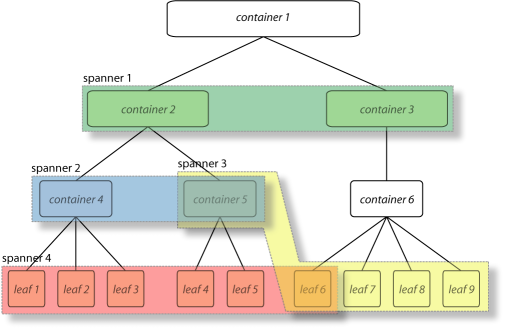
\includegraphics[scale=0.6]{include-container-spanner.png}
    \end{center}
\end{frame}

\begin{frame}{About the code base}

    \begin{itemize}
        \item 496 public classes
        \item 387 public functions
        \item 186,963 lines of code
        \item 9399 unit tests
        \item 10190 documentation tests
        \item 100\% free \& open source
        \item platform independent
        \item runs under both Python 2.7 and 3.3+
    \end{itemize}

\end{frame}

\section{Music}

\begin{frame}{A small concert}
    \begin{description}
        \item[2015] Josiah: \textbf{Invisible Cities (iii): Ersilia} \\
            for chamber orchestra
        \item[2015] Trevor: \textbf{Al-kitab al-khamr} \\
            for eleven players
        \item[2015] Josiah: \textbf{Invisible Cities (ii): Armilla} \\
            for viola duet
        \item[2014] Trevor: \textbf{Krummzeit} \\
            for seven players
    \end{description}
    \begin{center}
        Scores and source code are all available on GitHub.
    \end{center}
\end{frame}

\begin{frame}{Josiah's music}
    \begin{description}
        \item[2015] \textbf{Invisible Cities (iii): Ersilia} \\
            for chamber orchestra
        \item[2015] \textbf{Invisible Cities (ii): Armilla} \\
            for viola duet
        \item[2014] \textbf{Invisible Cities (i): Zaira} \\
            for eight players
        \item[2014] \textbf{Plague Water} \\
            for bari sax, e-guitar, piano and percussion
        \item[2011] \textbf{Aurora} \\
            for string orchestra
        \item[2010] \textbf{Lagartija} \\
            for mixed quartet
    \end{description}
\end{frame}

\begin{frame}{Trevor's music}
    \begin{description}
        \item[2015] \textbf{Al-kitab al-khamr} \\
            for eleven players
        \item[2015] \textbf{Ins Wasser eingeschrieben} \\
            for viola duet
        \item[2014] \textbf{Krummzeit} \\
            for seven players
        \item[2013] \textbf{Traiettorie inargentate} \\
            for cello
        \item[2011] \textbf{L'archipel du corps} \\
            for flute, guitar, accordion \& percussion
        \item[2009] \textbf{Mon seul désir} \\
            for flute, clarinet, violin \& cello
        \item[2008] \textbf{Lidércfény} \\
            for flute, violin \& piano
    \end{description}
\end{frame}

\begin{frame}{Jeff's music}
    \begin{description}
        \item[2015] \textbf{On the Behavior of Climbing Plants} \\ 
            for chamber orchestra
        \item[2013] \textbf{The World All Around} \\ 
            for Eb clarinet, prepared piano, and harp
        \item[2013] \textbf{+/-} \\ 
            for twenty french horns
        \item[2013] \textbf{Enfilade, Moses All, and Future Calendars} \\ 
            for carillon
        \item[2011] \textbf{Being Pollen} \\ 
            for solo percussion
    \end{description}
\end{frame}

%\begin{frame}{Other composers}
%    \begin{description}
%        \item Mike Solomon
%        \item Fredrik Wallberg
%        \item Oscar Dub
%        \item ???
%    \end{description}
%\end{frame}

%\begin{frame}{Analytics}
%    \begin{center}
%        Documentation visits by city since January 1st, 2015
%        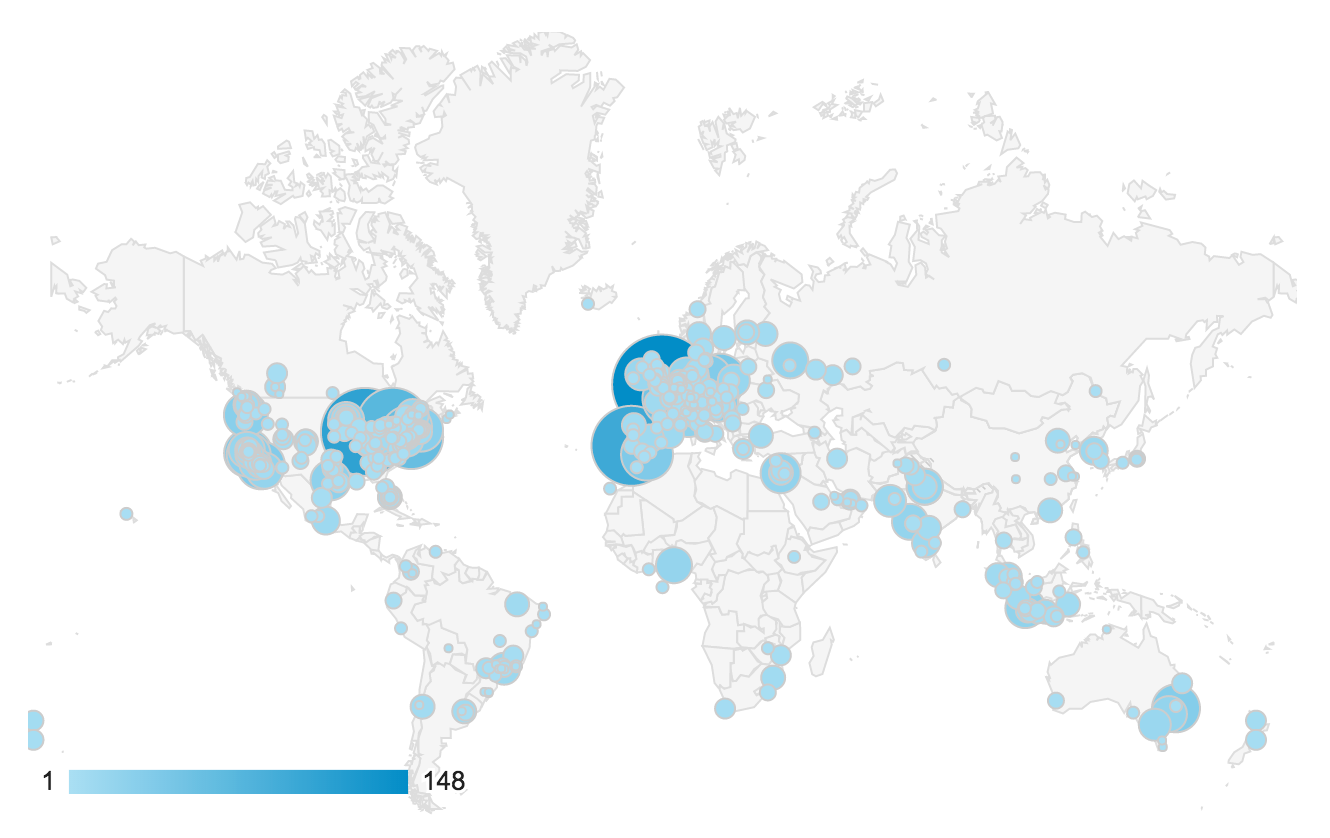
\includegraphics[scale=0.4, fbox]{analytics.png}
%    \end{center}
%\end{frame}

\section{Companion projects}

\begin{frame}{IPython}
Abjad integrates with \textbf{IPython} (\emph{ipython.org/}):

\begin{quote}
IPython is a command shell for interactive computing in multiple programming
languages, originally developed for the Python programming language, that
offers enhanced introspection, rich media, additional shell syntax, tab
completion, and rich history.
\end{quote}

IPython integration was spearheaded by \textbf{Prof. George K. Thiruvathukal}
(\emph{http://thiruvathukal.com}), Loyola University Chicago. 
\end{frame}

\begin{frame}{SASHA}

\textbf{Sasha} provides a database of saxophone multiphonic recordings and
their associated fingerings, allowing users to search for related multiphonics
by timbral, harmonic and idiomatic descriptors.

\begin{itemize}
    \item http://sasha.mbrsi.org
    \item http://github.com/josiah-wolf-oberholtzer/sasha
    \item Multiphonics performed by \textbf{Eliot Gattegno}
        (\emph{http://eliotgattegno.com})
\end{itemize}

Abjad acts together with many other Python libraries to handle programmatic
notational output, and to perform validation on musical queries.

\end{frame}

\section{Conclusion}

\begin{frame}{Conclusion}
The Abjad API for Formalized Score Control extends the Python programming
language with an open-source, object-oriented model of common-practice music
notation that enables composers to build scores through the aggregation of
elemental notation objects.
\end{frame}

\begin{frame}{Online Presence}

\textbf{Documentation} \\
http://projectabjad.org

\vfill{}

\textbf{GitHub Repository} \\
http://github.com/Abjad/abjad

\vfill{}

\textbf{User Mailing List} \\
http://groups.google.com/group/abjad-user

\end{frame}

\begin{frame}{TENOR 2015 (github.com/Abjad/tenor2015)}
    \begin{tabular}{cc}
    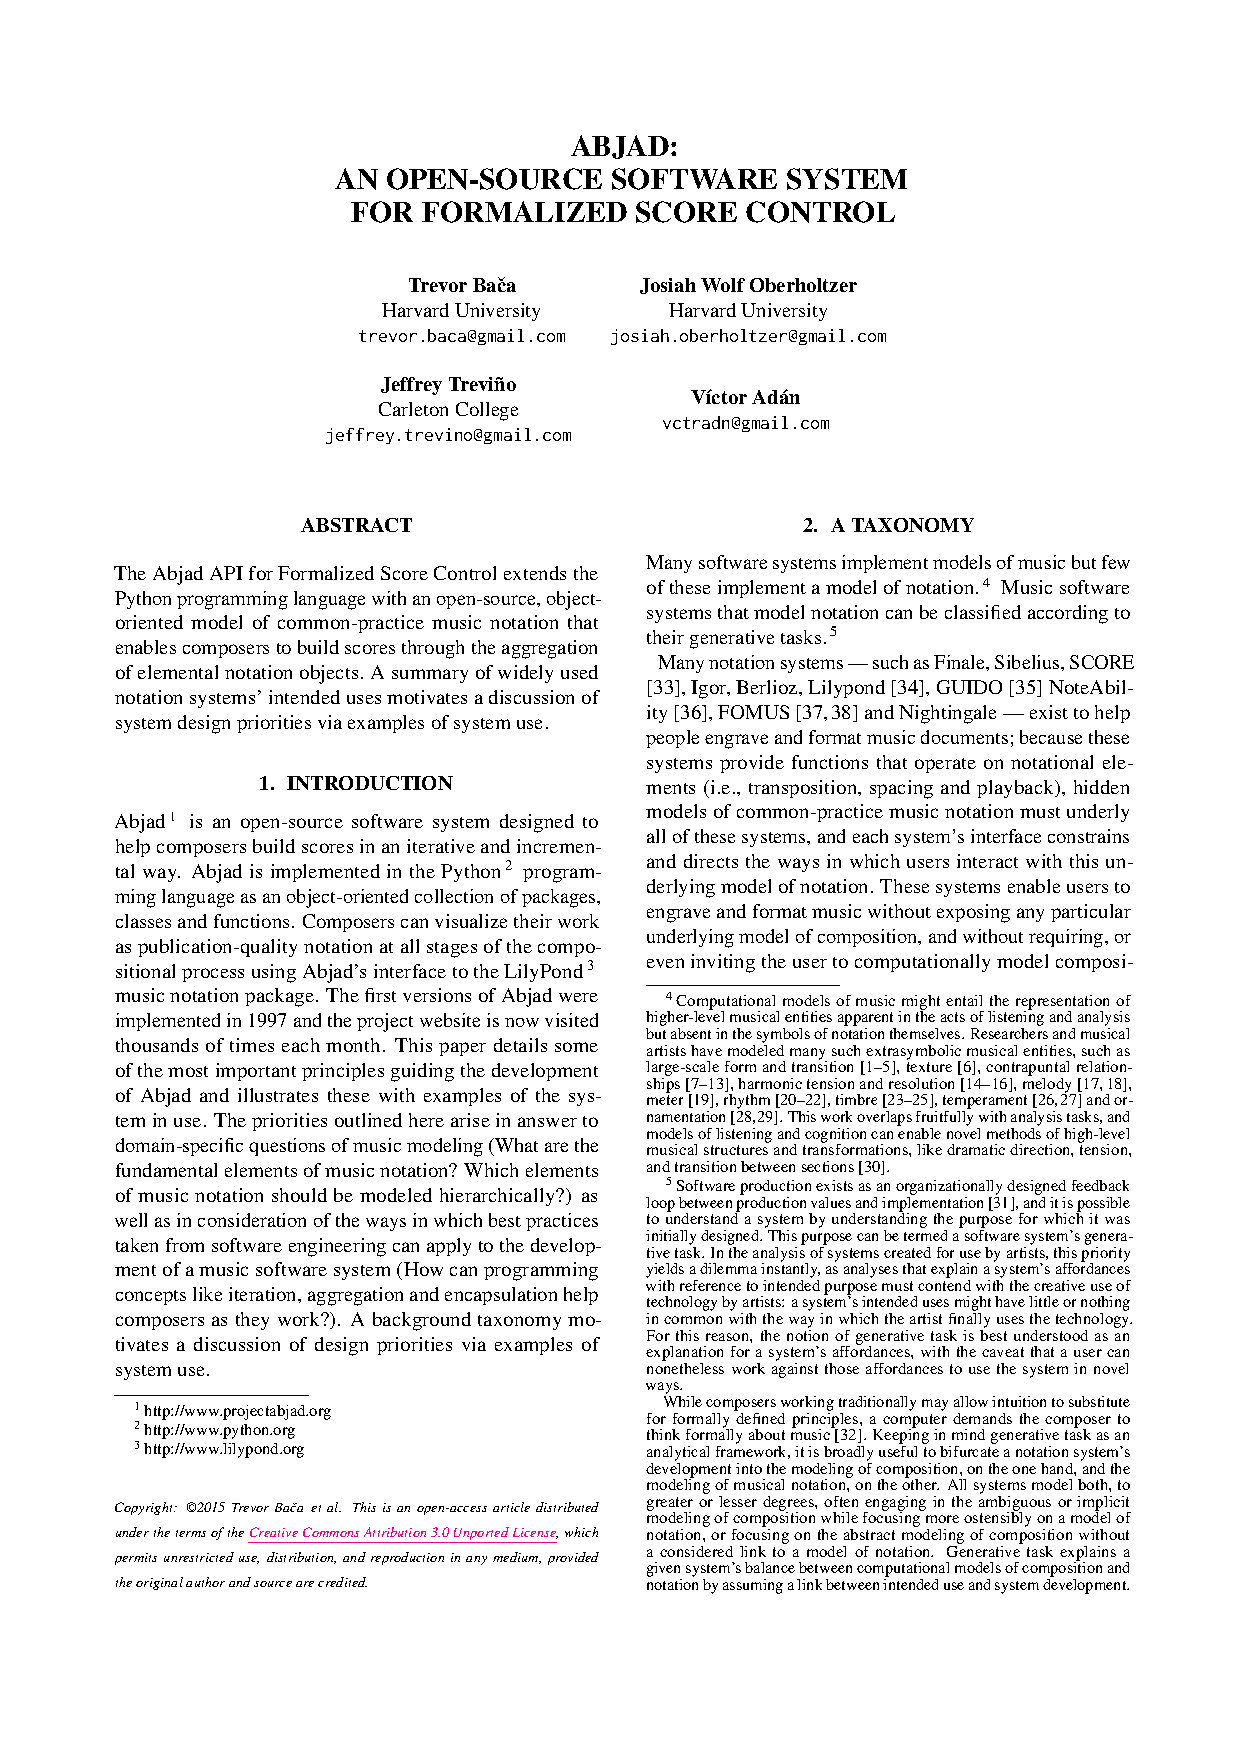
\includegraphics[
        page=1,
        scale=0.2,
        clip=true,
        fbox,
    ]{include-tenor2015.pdf}
    &
    \includegraphics[
        page=2,
        scale=0.2,
        clip=true,
        fbox,
    ]{include-tenor2015.pdf}
    \end{tabular}
\end{frame}


\begin{frame}{Personal Contacts}
    \begin{columns}[t,onlytextwidth]
        \column{.5\textwidth}
        \textbf{Trevor Ba\v{c}a}
        \begin{itemize}
            \item trevor.baca@gmail.com
            \item trevorbaca.com
            \item github.com/trevorbaca
        \end{itemize}
        \column{.5\textwidth}
        \textbf{Jeffrey Trevi\~{n}o}
        \begin{itemize}
            \item jeffrey.trevino@gmail.com
            \item jeffreytrevino.com
            \item github.com/jefftrevino
        \end{itemize}
    \end{columns}
    \vspace{\baselineskip}
    \textbf{Josiah Wolf Oberholtzer}
    \begin{itemize}
        \item josiah.oberholtzer@gmail.com
        \item josiahwolfoberholtzer.com
        \item github.com/josiah-wolf-oberholtzer
    \end{itemize}
\end{frame}

\end{document}